% ====================================================================
% VİZE RAPOR ŞABLONU – Türk Masalları Derlemesi Web Sayfası
% --------------------------------------------------------------------
% DERLEME: Overleaf'te Menu > Compiler > XeLaTeX (pdfLaTeX de çalışır).
%
% KURALLAR (şablonu kullanmadan önce okuyun):
%  1. Bölüm başlıklarını SİLMEYİN ve sırasını DEĞİŞTİRMEYİN.
%  2. [KÖŞELİ PARANTEZ] içindeki ve gri renkli açıklama metinlerini
%     kendi bilgilerinizle değiştirin; açıklama metinlerini silin.
%  3. MEBİS'e YALNIZCA bu raporun PDF'ini yükleyin.
%     ZIP ve HTML dosyası YÜKLEMEYİN. Tüm kontroller GitHub'dan yapılır.
%  4. Kapaktaki GitHub ve YouTube bağlantıları doğru ve tıklanabilir
%     olmalıdır. Teslimden önce PDF'teki bağlantılara tıklayıp deneyin.
%  5. Haftalık katkı tablosundaki görseller için resim dosyalarını
%     (hafta1.png, hafta2.png, ...) Overleaf projesine yükleyin.
%     Dosya adlarında boşluk ve Türkçe karakter kullanmayın.
%     Resim yoksa tabloda "görsel ekleyin" kutusu görünür.
%  6. Yapay zekâ kullandıysanız Bölüm 5'i doldurun.
% ====================================================================
\documentclass[12pt,a4paper]{article}

\usepackage{iftex}
\ifPDFTeX
  \usepackage[T1]{fontenc}
  \usepackage[utf8]{inputenc}
\else
  \usepackage{fontspec}
\fi
\usepackage[turkish]{babel}
\usepackage[margin=2.4cm]{geometry}
\usepackage{setspace}
\usepackage{graphicx}
\usepackage{booktabs}
\usepackage{longtable}
\usepackage{array}
\usepackage{colortbl}
\usepackage{xcolor}
\usepackage{enumitem}
\usepackage{listings}
\usepackage{amssymb}
\usepackage{caption}
\usepackage{fancyhdr}
\usepackage{hyperref}
\usepackage{float}
\onehalfspacing
\setlength{\parindent}{0pt}
\setlength{\parskip}{6pt}
\setlist{itemsep=2pt, topsep=4pt}
\hypersetup{colorlinks=true, linkcolor=blue!50!black, urlcolor=blue!50!black}

\definecolor{ana}{HTML}{14325C}
\definecolor{acik}{HTML}{EEF2F8}

\lstset{basicstyle=\ttfamily\small, backgroundcolor=\color{acik},
  frame=single, rulecolor=\color{ana}, breaklines=true,
  columns=fullflexible, keepspaces=true, showstringspaces=false}

\pagestyle{fancy}
\fancyhf{}
\fancyhead[L]{[PROJE ADI]}
\fancyhead[R]{Vize Raporu}
\fancyfoot[C]{\thepage}

% ---------- Yardımcı komutlar ----------
% Gri açıklama metni (silinecek yönergeler için)
\newcommand{\aciklama}[1]{{\color{gray}\itshape (#1)}}

% Haftalık tablo görseli: dosya yoksa "görsel ekleyin" kutusu çıkar
\newcommand{\haftagorsel}[1]{%
  \IfFileExists{#1}{%
    \includegraphics[width=\linewidth,height=4.2cm,keepaspectratio]{#1}%
  }{%
    \fbox{\parbox[c][2.6cm][c]{\dimexpr\linewidth-2\fboxsep-2\fboxrule\relax}{%
      \centering\small\color{gray} Ekran görüntüsü / görsel ekleyin\\ \texttt{#1}}}%
  }%
}
% Haftalık katılım kutuları (işaretlemek için $\square$ yerine $\boxtimes$ yazın)
\newcommand{\katilimkutulari}{\par\vspace{3pt}\small $\square$ Ders içinde katılım sergiledim\par $\square$ Telafi yaptım}

% Ek görsel: dosya yoksa hiçbir şey göstermez
\newcommand{\haftaek}[1]{%
  \IfFileExists{#1}{\\[4pt]\includegraphics[width=\linewidth,height=4.2cm,keepaspectratio]{#1}}{}%
}

% ---------- Kapak bilgileri ----------
\newcommand{\universite}{[ÜNİVERSİTE / BÖLÜM]}
\newcommand{\dersadi}{[DERS ADI]}
\newcommand{\hocaadi}{[ÖĞRETİM ÜYESİ]}
\newcommand{\ogrenciadi}{[AD SOYAD]}
\newcommand{\ogrencino}{[ÖĞRENCİ NUMARASI]}
\newcommand{\projeadi}{[PROJE ADI]}
% Bağlantıları tam adres olarak yazın (https:// ile başlayarak)
\newcommand{\githublink}{\url{https://github.com/KULLANICI-ADI/DEPO-ADI}}
\newcommand{\youtubelink}{\url{https://www.youtube.com/watch?v=VIDEO-KIMLIGI}}

\begin{document}

% ====================================================================
% KAPAK
% ====================================================================
\begin{titlepage}
\centering
\vspace*{1cm}
{\large \ İstanbul Medipol Üniversitesi / Görsel İletişim Tasarımı Bölümü }
\vspace{1.8cm}
{\Huge\bfseries\color{ana}  \ DİLDEN DİLE \par}
\vspace{1.8cm}
{\Large Türk Masalları Derlemesi Web Sayfası \par}
{\large Vize Raporu \par}
\vspace{1.8cm}
{\large \textbf{Ders:} \ Programlamaya Giriş \par}
{\large \textbf{Öğretim Üyesi:} \ Meral ŞENTÜRK \par}
\vspace{1.2cm}
{\large \textbf{Hazırlayan:} \ Rojin Esma BACNİ \par}
{large \textbf {Öğrenci No:} 86240047 \par}
\vspace{1.8cm}
\fbox{\parbox{0.88\linewidth}{\centering\vspace{6pt}
{\large\bfseries Proje Bağlantıları}\\[8pt]
\textbf{GitHub deposu:}\\ https://github.com/rojinbacni1/Turk-Masallari \\[8pt]
\textbf{YouTube sunum videosu:}\\ https://youtu.be/Gs1zI0n4LDw
\vspace{6pt}}}
\vfill
{\large \today \par}
\end{titlepage}

\tableofcontents
\newpage

% ====================================================================
\section{Giriş}
% ====================================================================
{Bu projenin temel amacı; Türk halk anlatı geleneğine ait seçilmiş masalları, kültürel dokuyu yansıtan okunabilir, estetik ve işlevsel bir web arayüzünde modern teknolojilerle bir araya getirmektir. Kullanıcının dikkatinin dağılmadan metne odaklanabilmesi amacıyla geleneksel kilim motifleri, lale bezemeleri ve dönemin atmosferini yansıtan bordo-altın renk paleti tercih edilmiştir. Ödev yönergeleri doğrultusunda derlemede kahramanlık masalından mizahi fıkraya, Dede Korkut anlatısından hayvan masallarına uzanan toplam 8 adet farklı eser yer almaktadır. Çalışmanın tüm gereksinimleri eksiksiz karşılanmış; tasarım ve stil kuralları harici bir dosya kullanılmadan doğrudan \texttt|<style>| etiketi altında içsel CSS olarak, etkileşim ve dinamik filtreleme mekanizmaları ise \texttt|<script>| etiketi altında içsel JavaScript olarak tek bir HTML dosyasında toplanmıştır. İnternet bağlantısı olmadan da tamamen çalışabilir şekilde kurgulanan sayfada; masal türü süzme, rastgele masal getirme, okuma süresi hesaplama, favori/okuma durumu takibi, gece modu ve sesli okuma gibi anlamlı JavaScript işlevleri geliştirilmiştir. Bu raporda; web sayfasının arayüz tasarım kararları, kullanılan içsel CSS ve JavaScript kodlarının çalışma mantığı, yararlanılan yapay zekâ araçlarının kapsamı ve haftalık ders içi katkı süreci ayrıntılı olarak belgelenmektedir. }

\subsection{Proje Özeti}
[\textbf{Dilden Dile: Türk Masalları Derlemesi}, Türk halk anlatı geleneğinden derlenen sekiz eseri tek bir HTML dosyasında toplayan, internet bağlantısı olmadan çalışabilen ve kullanıcı odaklı bir web sayfası projesidir. Arayüz tasarımı; kültürel atmosferi yansıtan bordo-altın renk paleti, SVG kilim motifleri ve metin okunabilirliğini artıran serfli yazı tipleriyle özgün olarak hazırlanmıştır. Ödev kurallarına uygun biçimde harici dosya kullanılmadan, tüm biçimlendirmeler \verb|<style>| etiketi altında içsel CSS, tüm etkileşimler ise \verb|<script>| etiketi altında içsel JavaScript ile kurgulanmıştır. Sayfada kullanıcının deneyimini kolaylaştırmak amacıyla masal türüne göre filtreleme, rastgele masal getirme, okuma süresi hesaplama, favori/okuma durumu takibi, gece modu ve sesli okuma gibi anlamlı JavaScript işlevleri geliştirilmiştir. ]

\subsection{Gereksinimlerin Karşılanması}
\begin{center}
\rowcolors{2}{acik}{white}
\begin{tabular}{@{}p{8.2cm}c@{}}
\toprule
\rowcolor{ana}\textcolor{white}{\textbf{Gereksinim}} & \textcolor{white}{\textbf{Durum}} \\
\midrule
Masal sayısı 8--12 arasında ([SAYI] masal)         & +\\
Tek HTML dosyası                                    & +\\
Stil kodları içsel (\texttt{<style>} içinde)        & +\\
Betik kodları içsel (\texttt{<script>} içinde)      & +\\
İnternetsiz açılıp çalışıyor                        & +\\
JavaScript sayfada anlamlı bir işlev görüyor        & +\\
Sayfa telefonda da düzgün görünüyor                 & -\\
\bottomrule
\end{tabular}
\end{center}
\aciklama{Karşıladığınız her satırın kutusunu $\boxtimes$ ile değiştirin.}

% ====================================================================
\section{Masalların Seçimi}
% ====================================================================
\aciklama{Hangi masalları, hangi ölçütlere göre seçtiniz? Tabloyu masal sayınıza göre
düzenleyin (en az 8, en fazla 12 satır). Kullandığınız kaynakları Kaynakça'ya yazın.}

\begin{longtable}{@{}cp{4cm}p{3cm}p{5.4cm}@{}}
\toprule
\textbf{No} & \textbf{Masal} & \textbf{Tür} & \textbf{Seçilme nedeni} \\
\midrule
\endhead
1 & Keloğlan ve Dev& Kahramanlık masalı& Türk masallarının en bilinen halk kahramanını temsil etmesi; kaba kuvvet yerine zekâ, kıvraklık ve cesaretin öne çıkarılması amacıyla seçilmiştir.\\
2 & Nasreddin Hoca Fıkraları& Fıkra / Mizahi Anlatı& Halk kültüründeki mizahi, düşündürücü ve hiciv dolu anlatı geleneğini derlemeye dahil etmek için seçilmiştir.\\
3 & Altın Saçlı Kız& Olağanüstü / Sihir Masalı& Geleneksel peri ve olağanüstü masal motiflerini, sabır ve hak arayışı temasını barındırdığı için seçilmiştir.\\
4 & Tahir ile Zühre& Halk Hikâyesi / Aşk Anlatıs& Türk halk hikâyesi ve Doğu aşk anlatısı geleneğini, bağlılık ve fedakârlık temasını temsil etmesi için seçilmiştir.\\
5 & Zümrüdü Anka& Mitolojik / Efsanevi Masal& Türk ve Doğu mitolojisindeki yeniden doğuş, rehberlik ve zorlukları aşma simgesini masallara taşıdığı için seçilmiştir.\\
6 & Gökten Üç Elma Düştü& Anonim Halk Masalı& Masal sonu tekerlemelerinin ve sözlü bitiriş ritüellerinin simgesel değerini sayfaya yansıtmak amacıyla seçilmiştir.\\
7 & Keloğlan ile Hacivat& Seyirlik / Gölge Oyunu Kaynaklı Masal& Geleneksel Türk temaşa sanatı figürleri ile halk masalı kahramanını bir araya getiren sözlü çatışma ve mizah kültürünü göstermek için seçilmiştir.\\
8 & Tepegöz& Destansı Anlatı& Dede Korkut anlatılarının epik ve mitolojik dilini, canavara karşı zekâ ve cesaretle verilen mücadeleyi temsil etmesi amacıyla seçilmiştir.\\
\bottomrule
\end{longtable}

% ====================================================================
\section{Tasarım Kararları}

\subsubsection{Tasarım Kararları ve Masal Okuma Amacına Hizmeti}

Web sayfasının arayüzü sıfırdan geliştirilmiş olup hazır bir web sitesi şablonu veya tema paketi kesinlikle kullanılmamıştır. Tasarımdaki her biçimsel ve yapısal tercih, kullanıcının dikkatini dağıtmadan doğrudan masal metnine odaklanmasını ve okuma sürecini rahatça yönetmesini sağlamak amacıyla şekillendirilmiştir: 

\begin{itemize}
    \item \textbf{Metin Genişliği ve Satır Ergonomisi:} Okuma alanının azami genişliği \verb|46rem| ile sınırlandırılmıştır. Bu sayede satırların aşırı uzaması engellenmiş, okuyucunun gözünün satır başından sonuna geçerken yorulmasının ve satır kaybetmesinin önüne geçilmiştir. 
    \item \textbf{Görsel Bezemelerin İşlevi:} Kullanılan SVG kilim bordürleri ve lale motifleri dikkat dağıtan birer süsleme değil; ana sayfa, başlıklar ve okuma metni arasında geçişi netleştiren hafif çizgisel ayraçlar olarak tasarıma dahil edilmiştir. 
    \item \textbf{Okuma Deneyimini Destekleyen Araçlar:} Kullanıcının fiziksel şartlarına uyum sağlamak için font boyutunu büyütüp küçülten butonlar (\verb|A+|, \verb|A-|), gece ortamında gözü dinlendiren karanlık mod (\verb|Gece|) ve yorulmadan anlatıyı takip etmeyi sağlayan \verb|Dinle| seçeneği eklenmiştir. 
    \item \textbf{Gezinme ve Takip Kolaylığı:} Kullanıcının sitede kaybolmaması adına ana sayfaya dönüş butonu, masallar arası hızlı geçiş sağlayan "Önceki / Sonraki masal" düğmeleri ve okuma durumunu kaydeden "Okudum" ile "Favorilere ekle" mekanizmaları arayüze entegre edilmiştir. 
    \item \textbf{Duyarlı (Responsive) Düzen:} Sayfa düzeni Flexbox ve CSS Grid yapılarıyla esnek tutulmuş; bilgisayar ekranında 4'lü vitrin şeklinde duran masal kartları, mobil ve dar ekranlarda otomatik olarak 2'li düzene geçerek her cihazda parmakla kolay tıklanabilir ve okunabilir kalmıştır.
\end{itemize}



\subsection{Konuya Uygunluk}
[Arayüzde tercih edilen renkler, tipografi ve görsel bezemeler, Türk halk anlatı geleneğinin masalsı ve köklü atmosferini doğrudan ekrana taşımak amacıyla seçilmiştir.

Arka plandaki derin bordo rengi ve çerçevelerdeki altın sarısı tonları, geleneksel Türk çadır ve saray kumaşlarının zenginliğini hissettirir. Bölüm ayraçlarında kullanılan geometrik kilim bordürleri ile başlıkları çevreleyen simetrik lale motifleri, Anadolu dokuma sanatına ve geleneksel tezhip motiflerine gönderme yapar. Okuma panelinde parşömen kâğıdı hissi veren krem zemin, koyu kahve mürekkep rengi ve ilk harfin büyük başladığı (drop cap) paragraf düzeni, kullanıcıya el yazması tarihi bir masal kitabını okuyormuş hissi kazandırarak temayla güçlü bir bağ kurar. 

 ]

\subsection{Renk Paleti ve Yazı Tipi}
\begin{center}
\rowcolors{2}{acik}{white}
\begin{tabular}{llp{6.4cm}}
\toprule
\rowcolor{ana}\textcolor{white}{\textbf{Ad}} & \textcolor{white}{\textbf{Kod}} & \textcolor{white}{\textbf{Nerede / neden kullandınız?}} \\
\midrule
Bordo & \#8e1b1b & Masalsı, derin ve geleneksel bir arka plan atmosferi oluşturmak için seçilmiştir.\\
Altın Sarısı & \#d9b878 & Başlıkları, çerçeveleri, kilim bordürlerini ve önemli butonları öne çıkarmak amacıyla kullanılmıştır.\\
Parşömen Kremi & \#f3e7c9 & Uzun okumalarda beyaz kağıt parlamasını engelleyen, gözü dinlendiren otantik bir okuma alanı sağlamak için tercih edilmiştir.\\
Koyu Kahve Mürekkep & \#2b1a12 & Krem zemin üzerinde net ve rahat bir okunabilirlik elde etmek için kullanılmıştır.\\
\bottomrule
\end{tabular}
\end{center}

\subsection{Okunabilirlik, Gezinme ve Duyarlı Tasarım}
\begin{itemize}
  \item \textbf{Okunabilirlik:} [Metin gövdesinde temel yazı boyutu \verb|1.2rem| (\verb|--boyut|) ve satır yüksekliği \verb|1.75| olarak belirlenerek ferah bir okuma ritmi yakalanmıştır. Okuma panelinin azami genişliği \verb|46rem| ile sınırlandırılmış; böylece satır uzunluğunun aşırı uzaması ve gözün satır takibinde yorulması engellenmiştir. Sayfa zemininde kullanılan sıcak parşömen kremi (\verb|#f3e7c9|) ile koyu kahve mürekkep rengi (\verb|#2b1a12|) arasındaki karşıtlık, beyaz ekran parlamasını önleyerek uzun soluklu okumalarda konforlu bir kontrast sağlamaktadır. Ayrıca arayüzdeki \verb|A+| ve \verb|A-| butonları sayesinde yazı boyutu kullanıcının tercihine göre dinamik olarak ayarlanabilmektedir.  ]
  \item \textbf{Gezinme:} [Kullanıcının istediği masala en kısa sürede ve zahmetsizce ulaşabilmesi hedeflenmiştir. Ana sayfada yer alan dinamik tür süzgeçleri sayesinde masallar kategorilerine göre tek tıkla filtrelenebilmekte, karar veremeyenler için "Bir masal seç bana" butonu rastgele bir masal açmaktadır. Masal kartlarına tıklandığında doğrudan ilgili okuma paneli açılmakta; panelin altındaki "Önceki" ve "Sonraki masal" butonlarıyla ana sayfaya dönmeden anlatılar arasında seri geçiş yapılabilmektedir. Üst kısımdaki "Ana sayfa" butonu ise tek tıkla vitrin görünümüne dönmeyi sağlamaktadır. ]
  \item \textbf{Duyarlı tasarım:} [Sayfa yerleşimi masaüstü, tablet ve mobil cihaz ekranlarına göre kademeli olarak uyarlanmıştır. Masal kartlarının listelendiği raf düzeni masaüstü geniş ekranlarda 4 sütunlu bir vitrin oluştururken, 900 piksel ve altındaki tablet ekranlarında 2 sütunlu ızgara yapısına geçmektedir. 420 piksel altındaki mobil telefon ekranlarında ise kart aralıkları, iç boşluklar (padding) ve başlık boyutları küçültülerek tek elle kaydırmaya ve dokunmatik kullanıma uygun, taşma yapmayan akıcı bir düzen sağlanmıştır.  ]
  \item \textbf{Tutarlılık:} [Başlık, boşluk ve renklerin kullanımı.]
\end{itemize}

\subsection{Ekran Görüntüleri}

\begin{center}
  \resizebox{11cm}{!}{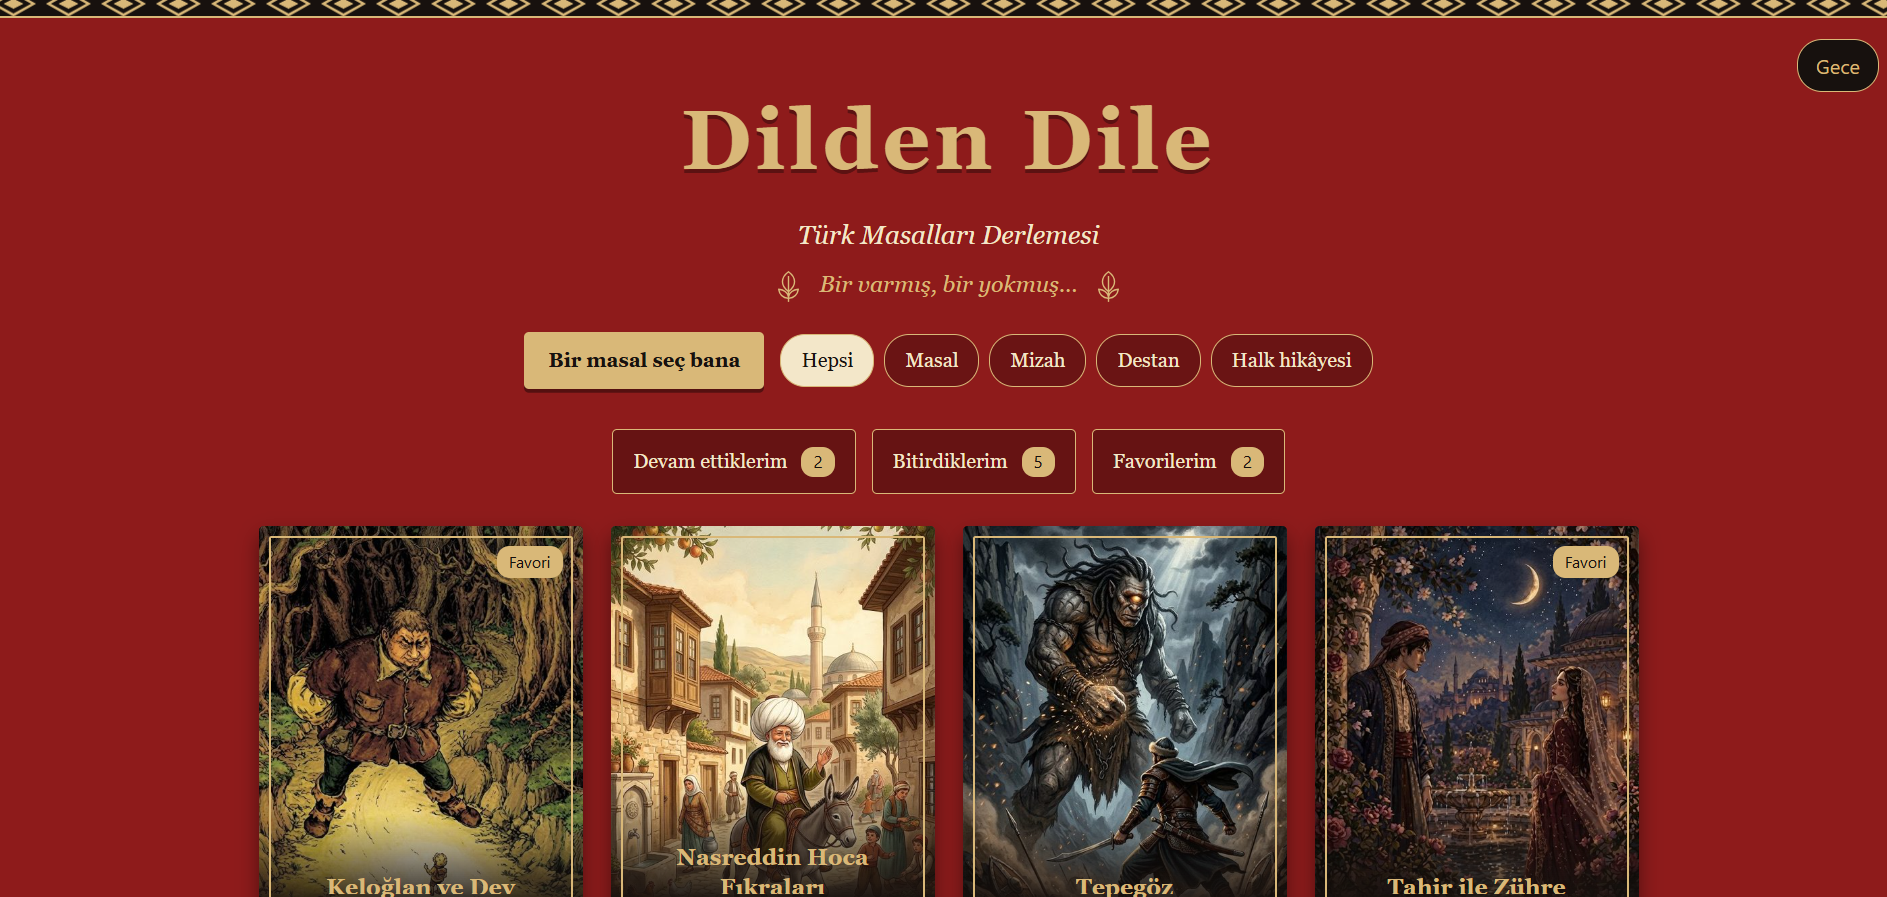
\includegraphics{ekran-masaustu.png}}

  \vspace{4pt}
  \small\textbf{Şekil 1:} Sayfanın bilgisayar görünümü
\end{center}

\vspace{0.4cm}

\begin{center}
  \resizebox{5.5cm}{!}{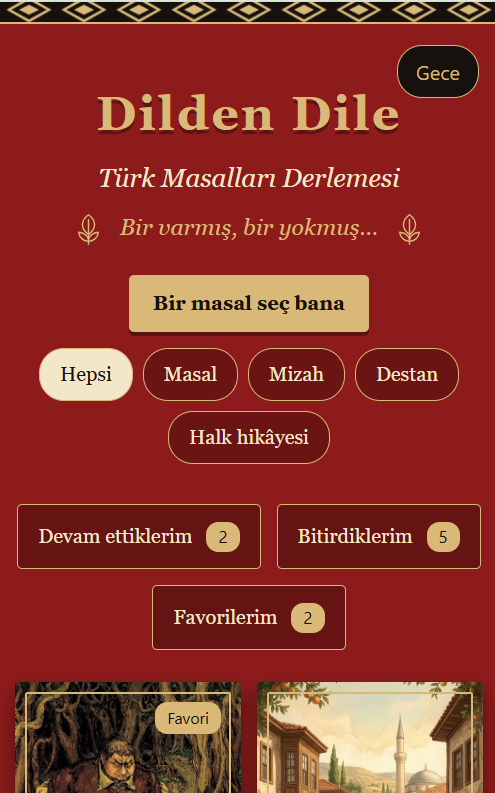
\includegraphics{ekran-mobil.png}}

  \vspace{4pt}
  \small\textbf{Şekil 2:} Sayfanın telefon görünümü
\end{center}
% ====================================================================
\subsection{HTML Yapisi}
Web sayfasi tek bir HTML dosyasi olarak hazirlanmis, harici hicbir sablon veya kutuphane kullanilmamistir. Semantik etiketler tercih edilerek yapi dort ana bolume ayrilmistir:
\begin{itemize}
  \item \textbf{header ve nav:} Logo, alt baslik, rastgele masal getiren buton ve JavaScript ile dinamik uretilen tur filtreleri yer alir.
  \item \textbf{main ve aside:} Masal kartlarinin listelendigi vitrin alani ile okuma durumu sayaclarini barindiran yan paneldir.
  \item \textbf{article id="okuma":} Masal secildiginde acilan, yazi boyutu ayarlari, sesli okuma ve tam metni iceren okuma alanidir.
  \item \textbf{footer:} Geleneksel kilim deseni seridi ile tasarimi tamamlayan alt bilgi alanidir.
\end{itemize}

\subsection{Icsel CSS}
Tum stil kurallari harici bir dosya acilmadan head icindeki style etiketine yazilmistir. Renk paleti ve temel yazi boyutu CSS degiskenleri (:root) uzerinden yonetilmis, boylece tek bir sinifla gece moduna gecis saglanmistir. Kart yerlesiminde esnek duzen (Flexbox) kullanilmis, media sorgulari ile masaustunde 4 sutun olan duzen mobilde tek ve cift sutunlu ergonomik akisa uyarlanmistir.

\begin{lstlisting}[caption={Icsel CSS Degiskenleri ve Grid Yapisi}]
:root {
  --zemin: #8e1b1b;
  --altin: #d9b878;
  --sayfa: #f3e7c9;
  --murekkep: #2b1a12;
  --boyut: 1.2rem;
}

body.gece {
  --zemin: #3b0f12;
  --sayfa: #1a1411;
  --murekkep: #efe3c8;
}

#okuma {
  max-width: 46rem;
  margin: 0 auto;
  line-height: 1.75;
}

@media (max-width: 900px) {
  .raf > .kart {
    width: calc((100% - 1.4rem) / 2);
  }
}
\end{lstlisting}

\subsection{Icsel JavaScript}
Etkilesimler kutuphanesiz saf JavaScript ile script etiketi icinde cozulmustur. 8 adet masal verisi; id, baslik, tur, sure ve metin alanlariyla bir nesne dizisi icinde tutulur. Sayfa acildiginda kartlar ve tur butonlari DOM uzerine dinamik basilir. Okundu durumu ve favoriler kullanicinin tarayici hafizasinda (localStorage) saklanir. Sesli okuma icin Web Speech API kullanilmistir.

\begin{lstlisting}[caption={Icsel JavaScript Masal Dizisi ve Okuma Fonksiyonu}]
const masallar = [
  { id: 1, baslik: "Keloglan ile Dev", tur: "Masal", sure: 4 },
  { id: 2, baslik: "Nasreddin Hoca", tur: "Mizah", sure: 2 }
];

function masalAc(id) {
  const secilen = masallar.find(m => m.id === id);
  document.querySelector(".raf").hidden = true;
  document.getElementById("okuma").hidden = false;
  document.getElementById("baslik").textContent = secilen.baslik;
  window.scrollTo(0, 0);
}
\end{lstlisting}

\subsection{Sayfanin Ozellikleri}
\begin{itemize}
  \item \textbf{Tur Filtreleme:} Masallari turlerine gore dinamik suzme.
  \item \textbf{Rastgele Secim:} Kararsiz okurlar icin tek tikla masal getirme.
  \item \textbf{Yazi Boyutu Ayari:} A+ ve A- butonlari ile kisisellestirilebilir tipografi.
  \item \textbf{Gece Modu:} Dusuk kontrasta gecerek gozu yormayan karanlik tema.
  \item \textbf{Sesli Okuma:} Masal metnini seslendiren erisilebilirlik destegi.
  \item \textbf{Ilerleme Takibi:} Okunan ve favori masallari tarayici hafizasinda tutma.
\end{itemize}


% ====================================================================
\section{Yapay Zekâ Kullanımı}
% ====================================================================
GÖRSEL PROMPTLAR ( ChatGBT)
1. Keloğlan ve Div
 
Create a vertical rectangular book cover illustration inspired by the traditional Turkish folktale “Keloğlan ve Div.” Depict Keloğlan as a clever, humble young Anatolian peasant boy with a completely bald head, wearing traditional simple village clothing, a cream shirt, a dark red vest, and loose brown trousers. He stands fearlessly before an enormous, mysterious giant emerging from an ancient forest. The giant should appear powerful and intimidating but fantastical rather than horrifying. Include towering trees, distant Anatolian mountains, atmospheric mist, and subtle golden light breaking through the clouds. Use deep forest green, earthy brown, muted burgundy, and antique gold. Art style: sophisticated hand-painted storybook illustration, rich painterly textures, subtle vintage paper grain, intricate details, dramatic cinematic lighting, Turkish folklore atmosphere, beautiful editorial book-cover composition. Vertical 2:3 aspect ratio, strong central composition, visually clear at small thumbnail size. No text, no letters, no typography, no watermark, no mockup.

2. Nasreddin Hoca Fıkraları
 
Create a vertical rectangular illustrated book cover inspired by the humorous traditional stories of Nasreddin Hoca. Depict a wise, cheerful elderly Anatolian man with a white turban, a traditional robe, and a playful, knowing smile, riding a small gray donkey through a charming historical Anatolian village. His expression should communicate intelligence, gentle humor, and mischief. Include stone houses, an old village square, distant minarets, warm sunlight, and small environmental details that evoke everyday village life. Use warm ochre, terracotta, olive green, cream, and muted turquoise. Art style: detailed hand-painted Turkish folklore storybook illustration, elegant painterly brushwork, subtly aged paper texture, charming expressive character design, warm cinematic lighting, sophisticated editorial composition. Vertical 2:3 aspect ratio, balanced composition, suitable for a cohesive Turkish folktale book collection. No text, no letters, no typography, no watermark, no mockup.

3. Tepegöz — Dede Korkut
 
Create a vertical rectangular book cover illustration inspired by Tepegöz from the Turkish epic tradition of Dede Korkut. Depict a colossal, mythical one-eyed giant with rough skin, tangled dark hair, and a powerful silhouette emerging among enormous rocky formations. His single eye should be clearly visible and glowing faintly amber. In the foreground, a small Oghuz warrior holding a sword faces the giant with courage, emphasizing the dramatic difference in scale. Surround them with rugged Anatolian mountains, storm clouds, drifting dust, and a narrow beam of light illuminating the confrontation. Use charcoal black, deep midnight blue, stone gray, burnt umber, and restrained amber highlights. Art style: epic hand-painted fantasy illustration, historical Turkish folklore inspiration, textured brushwork, aged parchment grain, atmospheric depth, dramatic chiaroscuro, serious literary book-cover aesthetic. Vertical 2:3 aspect ratio. Powerful composition, detailed but readable at thumbnail size. No graphic violence, no text, no letters, no typography, no watermark, no mockup.

4. Tahir ile Zühre
 
Create a vertical rectangular illustrated book cover inspired by the traditional Turkish love story “Tahir ile Zühre.” Depict Tahir and Zühre as two young lovers standing apart in a beautiful historical Anatolian palace garden, looking at each other with deep affection and longing. Tahir wears elegant but understated traditional clothing, while Zühre wears a flowing burgundy dress with delicate embroidered details and a graceful veil. Frame them with flowering branches, roses, an ornate stone fountain, and distant palace architecture. A luminous crescent moon and scattered stars illuminate the quiet garden, creating a romantic atmosphere touched by melancholy. Use midnight blue, dusty rose, muted burgundy, soft lavender, and antique gold. Art style: poetic hand-painted storybook illustration, delicate painterly textures, intricate botanical details, subtle vintage paper grain, cinematic moonlight, elegant Turkish literary romance aesthetic. Vertical 2:3 aspect ratio, graceful central composition, visually harmonious as part of a Turkish folklore book collection. No text, no letters, no typography, no watermark, no mockup.

5. Gökten Düşen 3 Elma
  
Create a vertical rectangular book cover illustration inspired by the traditional Turkish fairy-tale ending “Gökten Üç Elma Düşmüş.” Depict three beautiful luminous apples falling gently from a magical night sky into an enchanted Anatolian garden. One apple is deep ruby red, one is golden amber, and one is soft crimson with delicate golden highlights. Surround them with tiny sparkling stars, delicate flowering branches, an ancient stone fountain, and a distant traditional Anatolian village beneath a deep twilight sky. The scene should evoke the magic of storytelling, happiness, hope, and the timeless tradition of Turkish folk tales. Use deep emerald green, midnight blue, warm cream, ruby red, and antique gold. Art style: sophisticated hand-painted Turkish fairy-tale book illustration, rich painterly textures, subtle vintage paper grain, delicate ornamental details inspired by traditional Anatolian art, magical cinematic lighting, elegant editorial composition. Vertical 2:3 aspect ratio, clear central composition, suitable for a cohesive Turkish folktale book collection. No text, no letters, no typography, no watermark, no mockup.

6. Zümrüdüanka
 
Create a vertical rectangular fantasy book cover inspired by Zümrüdüanka, the legendary magnificent bird associated with Turkish and wider regional folklore traditions. Depict an enormous mythical phoenix with emerald-green, turquoise, and golden feathers, spreading its majestic wings above a dramatic landscape of ancient mountains and clouds. Its feathers should shimmer with subtle jewel-like details, while warm golden light radiates from behind its body. Below, tiny distant ruins and winding mountain paths suggest a mysterious legendary world. The bird should appear noble, ancient, powerful, and magical rather than cartoonish. Use emerald green, deep teal, midnight blue, antique gold, and luminous amber. Art style: luxurious hand-painted fantasy storybook illustration, intricate feather detailing, painterly textures, atmospheric clouds, subtle vintage paper grain, dramatic cinematic lighting, sophisticated literary book-cover design. Vertical 2:3 aspect ratio, centered majestic bird, beautiful silhouette and rich visual depth. No text, no letters, no typography, no watermark, no mockup.

7. Altın Saçlı Kız
 
Create a vertical rectangular storybook cover inspired by the traditional fairy-tale motif of “Altın Saçlı Kız.” Depict a young woman with extraordinarily long, luminous golden hair flowing naturally in the breeze, standing in an enchanted garden surrounded by delicate wildflowers, climbing vines, and ancient trees. She wears an elegant cream-colored traditional fairy-tale dress with fine embroidered details. In the distance, an old stone castle rises above a peaceful river, partially hidden by morning mist. Sunlight filters through the trees, illuminating her hair and creating a magical golden halo without making the image overly bright. Use muted sage green, antique gold, warm ivory, soft sky blue, and subtle dusty rose. Art style: refined hand-painted fairy-tale illustration, delicate brushwork, intricate botanical textures, softly aged paper grain, elegant natural lighting, timeless literary book-cover aesthetic. Vertical 2:3 aspect ratio, graceful composition, detailed but visually clear at small size. No text, no letters, no typography, no watermark, no mockup.
8. Karagöz ile Hacivat
 
Create a vertical rectangular illustrated book cover inspired by the traditional Turkish shadow theatre of Karagöz and Hacivat. Depict the two iconic shadow-play characters facing each other in expressive conversation behind a softly glowing translucent theatre screen. Karagöz should have his recognizable dark silhouette, expressive eyes, and traditional costume; Hacivat should wear his distinctive tall headwear and elegant traditional clothing. Their poses should suggest a lively, humorous exchange. Include a subtle view of the wooden puppet-theatre frame, warm lantern light, and delicate decorative patterns inspired by traditional Ottoman-era visual arts. Use burnt orange, deep burgundy, warm cream, dark brown, and antique gold. Art style: artistic reinterpretation of traditional Turkish shadow puppetry, layered translucent colors, handcrafted cut-out textures, intricate ornamental details, subtle vintage paper grain, warm theatrical lighting, sophisticated editorial illustration. Vertical 2:3 aspect ratio, visually balanced composition, authentic cultural atmosphere, suitable for a unified Turkish folklore book collection. No text, no letters, no typography, no watermark, no mockup.


 
KOD ( CLAUDE) 

Bu projenin web geliştirme sürecinde yapay zekâ desteği olarak Claude modelinden yararlanılmıştır. Web sitesinin genel HTML iskeletinin oluşturulması, metin ve kutu hiyerarşisini kuran CSS kurallarının yapılandırılması ve DOM manipülasyonu sağlayan JavaScript fonksiyonlarının kodlanması Claude desteğiyle gerçekleştirilmiştir. Sayaç mekanizması ve etkileşimli buton mantığı yapay zekâ yönlendirmeleriyle kurulmuş; karşılaşılan sözdizimi ve çalışma hataları yine bu modelle ayıklanmıştır. Üretilen kodlar doğrudan kopyalanıp bırakılmamış, proje gereksinimlerine göre incelenip değişken ve stil düzenlemeleri bizzat tarafımdan yapılmış, sayfanın test ve çalıştırma süreçleri manuel olarak yürütülmüştür.

 
% ====================================================================
\section{Haftalık Katkılar}
% ====================================================================
\aciklama{Her hafta ders içinde yaptığınız çalışmayı kısaca yazın (2--4 cümle). Hangi
özelliği eklediğinizi ya da neyi düzelttiğinizi belirtin ve ilgili commit mesajını
ya da bağlantısını ``Commit'' satırına yazın. Her satıra ekran görüntüsü ekleyin:
resimleri \texttt{hafta1.png}, \texttt{hafta2.png}, \ldots{} adıyla Overleaf
projesine yükleyin. Aynı haftaya ikinci bir görsel eklemek için
\texttt{hafta1b.png} gibi bir dosya yükleyin; kendiliğinden görünür.
Her haftanın altındaki kutulardan o hafta için geçerli olanı $\boxtimes$ ile
işaretleyin: dersin kendisinde katılım gösterdiyseniz ``Ders içinde katılım
sergiledim'', o haftayı sonradan tamamladıysanız ``Telafi yaptım''. Telafi
yaptıysanız yapılan çalışmanın metninde bunu açıkça belirtin.}

\begin{longtable}{@{}>{\raggedright\arraybackslash}p{1.7cm}%
                    >{\raggedright\arraybackslash}p{6.4cm}%
                    >{\centering\arraybackslash}p{6cm}@{}}
\toprule
\rowcolor{ana}\textcolor{white}{\textbf{Hafta}} & \textcolor{white}{\textbf{Yapılan çalışma}} & \textcolor{white}{\textbf{Görsel}} \\
\midrule
\endfirsthead
\toprule
\rowcolor{ana}\textcolor{white}{\textbf{Hafta}} & \textcolor{white}{\textbf{Yapılan çalışma}} & \textcolor{white}{\textbf{Görsel}} \\
\midrule
\endhead
\bottomrule
\endfoot

1. Hafta\newline [16.10.2026] &
İlk web sayfası olan WorldWideWeb projesinin HTML ve içsel CSS kuralları kullanılarak yeniden inşası yapılmıştır. Temel semantik etiketler ve tipografi özellikleri düzenlenmiştir. İlgili haftanın çalışması ders saatinde bulunulamadığı için telafi kapsamında sonradan tamamlanmıştır.\newline
Commit: \texttt{feat: WorldWideWeb arayuz yeniden insasi ve temel CSS}\newline
[ ] Ders içinde katılım sergiledim \quad [X] Telafi yaptım &
\haftagorsel{hafta1.png} \\
\midrule
2. Hafta\newline [23.10.2026] &
Little Miss Sunshine filmi için başlık hiyerarşileri, bağlantılar ve alıntı blokları içeren bir inceleme sayfası hazırlanmıştır. Harici görsel bağlantısı eklenmiş ve içsel CSS ile metin-kutu hiyerarşisi biçimlendirilmiştir. İlgili haftanın çalışması ders saatinde bulunulamadığı için telafi kapsamında sonradan tamamlanmıştır.\newline
Commit: \texttt{feat: Little Miss Sunshine film inceleme ve karakter sayfasi}\newline
[ ] Ders içinde katılım sergiledim \quad [X] Telafi yaptım &
\haftagorsel{hafta2.jpg}\haftaek{hafta2b.png} \\
\midrule
3. Hafta\newline [30.09.2026] &
JavaScript DOM olayları kapsamında tıklama, çift tıklama, fare hareketleri ve girdi okuma mekanizmaları kodlanmıştır. Sayfa içi etkileşimler ve yeni sekme açma fonksiyonları ders saatinde test edilerek arayüze bağlanmıştır.\newline
Commit: \texttt{feat: Temel DOM olay dinleyicileri ve girdi islemleri}\newline
[X] Ders içinde katılım sergiledim \quad [ ] Telafi yaptım &
\haftagorsel{hafta3.jpg}\haftaek{hafta3b.png} \\
\midrule
4. Hafta\newline [07.10.2026] &
JavaScript değişkenleri kullanılarak sayısal bir sayaç mekanizması geliştirilmiştir. Buton tıklamasıyla sayıyı 5 artıran ve başlangıç durumuna sıfırlayan DOM güncellemeleri ders saatinde başarıyla kodlanmıştır.\newline
Commit: \texttt{feat: Sayac mekanizmasi ve dinamik DOM guncellemesi}\newline
[X] Ders içinde katılım sergiledim \quad [ ] Telafi yaptım &
\haftagorsel{hafta4.jpg}\haftaek{hafta4b.png} \\
\midrule
5. Hafta\newline [14.10.2026] &
Buton tıklamasıyla sayfa yönlendirmesi ve 4 kartlı interaktif renk eşleme hafıza oyunu geliştirilmiştir. Dizi yönetimi, zamanlayıcı ve kart eşleşme koşulları telafi kapsamında sonradan kodlanarak tamamlanmıştır.\newline
Commit: \texttt{feat: Sayfa yonlendirme ve interaktif kart esleme oyunu}\newline
[ ] Ders içinde katılım sergiledim \quad [X] Telafi yaptım &
\haftagorsel{hafta5.jpg}\haftaek{hafta5b.png} \\
\midrule
6. Hafta\newline [21.10.2026] &
Harici CSS dosyasının HTML sayfasına link etiketiyle bağlanması ve sayfa düzeni uygulanmıştır. JavaScript koşullu durumları (if/else) ile buton üzerinden arka plan rengi değiştirme yapısı telafi kapsamında sonradan kodlanmıştır.\newline
Commit: \texttt{feat: External CSS baglantisi ve dinamik arka plan degisimi}\newline
[ ] Ders içinde katılım sergiledim \quad [X] Telafi yaptım &
\haftagorsel{hafta6.jpg}\haftaek{hafta6b.png} \\
\bottomrule
\end{longtable}

\section{Test ve Değerlendirme}
% ====================================================================
\aciklama{Sayfayı hangi tarayıcı ve cihazlarda denediniz? Çalışmayan bir özellik
olduysa dürüstçe yazın ve nedenini açıklayın.}

\begin{center}
\rowcolors{2}{acik}{white}
\begin{tabular}{@{}p{6cm}p{3.4cm}p{3.4cm}@{}}
\toprule
\rowcolor{ana}\textcolor{white}{\textbf{Özellik}} & \textcolor{white}{\textbf{Bilgisayar}} & \textcolor{white}{\textbf{Telefon}} \\
\midrule
Arayüz düzeni ve CSS stilleri & Çalışıyor & Sorun var \\
DOM olayları ve buton etkileşimleri & Çalışıyor & Sorun var \\
Sayaç ve dinamik script fonksiyonları & Çalışıyor & Sorun var \\
\bottomrule
\end{tabular}
\end{center}

\textbf{Denenen tarayıcılar:} Google Chrome (Masaüstü), Apple Safari (iOS / iPhone)

\vspace{0.5em}
\noindent\textbf{Değerlendirme ve Karşılaşılan Sorunlar:}\newline
Sayfa masaüstü ortamında Google Chrome tarayıcısında test edilmiş; HTML yapısı, içsel CSS stilleri ve tüm JavaScript fonksiyonları (DOM olayları, sayaç mekanizması) hatasız bir şekilde çalışmıştır. 

iPhone (iOS Safari) ortamında yapılan testlerde sayfa açılamamış ve çalıştırılamamıştır. Bu durumun temel nedeni projenin yerel dizin üzerinden çalıştırılması, iOS Safari'nin katı yerel dosya güvenlik kısıtlamaları (\texttt{file://} protokolü engeli) ve mobil dokunmatik olaylara (\textit{touch events}) yönelik özel bir viewport/script uyarlaması yapılmamış olmasıdır. Projenin mobil uyumluluğu için ilerleyen süreçte canlı sunucuya (GitHub Pages vb.) alınması ve dokunmatik etkileşimlerin desteklenmesi gerekmektedir.

% ====================================================================
\section{Sunum Videosu}
% ====================================================================
\begin{center}
\begin{tabular}{@{}ll@{}}
\textbf{Video süresi:} & 12 dakika\\
\textbf{Görünürlük:} & Listelenmemiş\\
\textbf{Bağlantı:} & https://youtu.be/Gs1zI0n4LDw\\
\end{tabular}
\end{center}

\subsection{Video Kontrol Listesi}
\aciklama{Teslimden önce hepsini kontrol edin ve kutuları $\boxtimes$ ile işaretleyin.}
\begin{itemize}
  \item[[X]] Süre 12--18 dakika aralığında.
  \item[[X]] Sunum boyunca kameram açık, yüzüm görünüyor.
  \item[[X]] Görünürlük \textbf{Listelenmemiş} (ya da Herkese açık); \textbf{Özel} değil.
  \item[[X]] Bağlantıyı gizli pencerede açtım, video oynuyor.
  \item[[X]] Videoyu baştan sona izledim; ses ve kamera tüm sunumda var.
  \item[[X]] Kapaktaki bağlantı ile bu bölümdeki bağlantı aynı.
\end{itemize}

% ====================================================================
\section{Sonuç ve Kendi Değerlendirmem}
% ====================================================================
\aciklama{Projeden ne öğrendiniz? En çok nerede zorlandınız ve nasıl çözdünüz? İleride
neyi geliştirirdiniz? 6--10 cümle yeterlidir.}

Bu proje sürecinde semantik HTML yapısı kurmayı, içsel CSS ile tipografik ve görsel hiyerarşi oluşturmayı ve temel JavaScript ile DOM manipülasyonu gerçekleştirmeyi deneyimledim. Tasarlanan sayfanın tek bir dosya içinde harici kütüphane gerektirmeden çalışabilir olmasını sağlamak, web geliştirmenin temel mantığını kavramamda etkili oldu. Proje geliştirirken en çok JavaScript olay dinleyicilerinin (event listener) DOM elemanlarıyla senkronize çalışması ve sayaç mekanizmasında karşılaşılan durum yönetiminde zorlandım. Bu teknik engelleri tarayıcı geliştirici konsolunu aktif kullanarak, adım adım testler yaparak ve yapay zekâ desteğiyle kod mantığını ayıklayarak çözdüm. Ayrıca mobil tarayıcı kısıtlamaları ve yerel dosya güvenliği konusunda pratik tecrübe kazandım.. Ek olarak, masal seçimi arayüzüne daha zengin görsel animasyonlar ve ses efektleri entegre ederek kullanıcı deneyimini güçlendirmeyi planlardım.

% ====================================================================
\section{Kaynakça}
% ====================================================================
\begin{thebibliography}{9}
\bibitem{k1} İSEV. (2015). \emph{Keloğlan Masalları: Dev ile Keloğlan}. \url{https://www.isev.org.tr/wp-content/uploads/2015/12/keloglan_isev.pdf}, erişim tarihi: 29 Ekim 2026.
\bibitem{k2} Akşehir Belediyesi. \emph{Nasreddin Hoca Fıkraları (Fıkra 1--10)}. \url{http://aksehir.bel.tr/fikralar.pdf}, erişim tarihi: 29 Ekim 2026.
\bibitem{k3} Masal Dünyası. \emph{Dede Korkut -- Tepegöz}. \url{https://masal-dunyasi.vercel.app/masallar/dede-korkut-tepegoz}, erişim tarihi: 2 Kasım 2026.
\bibitem{k4} “Tahir ile Zühre”, Derki, https://derki.net/tr/product/964/tahir-ile-zuhre (erişim: 2 Kasım 2026).
\bibitem{k5} Kaynak: “Gökten Düşen Üç Elma Masalı”, Masal Oku, https://www.masaloku.net/gokten-dusen-uc-elma/ (erişim: 2 Kasım 2026).
\bibitem{k6} Kaynak: Bahar Arvasi, “Zümrüdüanka Kuşu”, Masal Dergisi, sayı 12, 2022, https://www.masaldergisi.com/sayilar/2022/sayi-12/zumruduanka-kusu/ (erişim: 2 Kasım 2026). Yazarın dayandığı kaynaklar: Tahir Alangu, Billur Köşk Masalları, YKY, 2022; Eflatun Cem Güney, Zümrütanka, Yelkovan Dizisi, 2007.
\bibitem{k7}Kaynak: “Altın Saçlı Kız Masalı”, Masal Oku, https://www.masaloku.net/altin-sacli-kiz-masali/ (erişim: 2 Kasım 2026).
\bibitem{k8}Kaynak: “Karagöz – Hacivat Perde Gazeli”, “Bayramlaşma Bayramı”, “Kolay Şiir”, Masal Oku, Karagöz ve Hacivat bölümü, https://www.masaloku.net/kategori/karagoz-ve-hacivat/ (erişim: 2 Kasım 2026).
\end{thebibliography}

% ====================================================================
\appendix
\section{Teslim Kontrol Listesi}
% ====================================================================
\aciklama{Teslim etmeden önce işaretleyin. Bu sayfayı teslim edilen PDF'te bırakabilirsiniz.}
\begin{itemize}[label={}]
  \item + MEBİS'e \textbf{yalnızca bu raporun PDF'ini} yükleyeceğim. ZIP ve HTML dosyası yüklemeyeceğim.
  \item  + Dosya adı \texttt{OgrenciNo\_AdSoyad\_vize.pdf} biçiminde.
  \item  +Kapaktaki GitHub ve YouTube bağlantıları doğru; PDF'te tıklayıp denedim.
  \item  +GitHub deposunda web sayfası (tek \texttt{.html}), rapor PDF'i, \texttt{.tex} kaynakları ve \texttt{README.md} var.
  \item  + GitHub deposu \textbf{herkese açık} (ya da öğretim üyesine erişim verdim).
  \item  + Çalışmamın son hâli teslim saatinden \textbf{önce} depoya gönderildi (sonraki commitler değerlendirilmez).
  \item  + Sayfa içsel CSS ve içsel JavaScript kullanıyor, harici dosya gerektirmiyor.
  \item  + Hazır taslak kullanmadım; yapay zekâ kullandıysam Bölüm 5'i doldurdum.
  \item  +Çalışmanın mantığını sunumda anlatabilirim.
\end{itemize}

\end{document}